\documentclass[12pt, a4paper, simple]{eskdtext}

\usepackage{hyperref}
\usepackage{_env/gpi_global.env}
\usepackage{_env/gpi_report.env}
\usepackage{_sty/gpi_lst}
\usepackage{_sty/gpi_toc}
\usepackage{_sty/gpi_t}
\usepackage{_sty/gpi_p}
\usepackage{_sty/gpi_u}

% Переменные
\def \gpiDocNum {3}
\def \gpiTopicRep {Планирование создания программных элементов (ПЭ) для
автоматизированной системы обработки информации (АСОИ)}

% Код
% \ESKDletter{О}{Л}{Р}
% \def \gpiDocTypeNum {81}
% \def \gpiDocVer {00}
% \def \gpiCode {\ESKDtheLetterI\ESKDtheLetterII\ESKDtheLetterIII.\gpiStudentGroupName\gpiStudentGroupNum.\gpiStudentCard-0\gpiDocNum~\gpiDocTypeNum~\gpiDocVer}

\def \gpiDocTopic {Отчёт лабораторной работы №\gpiDocNum}

% колонтитулы
\usepackage{fancybox, fancyhdr}
\fancypagestyle{plain}
{
    \renewcommand{\footrulewidth}{0pt}          % Толщина отделяющей полоски снизу
    \renewcommand{\headrulewidth}{0pt}          % Толщина отделяющей полоски сверху
    \fancyhead[C]{ }                            % Коллонтитул сверху
    \fancyfoot[C]{\hfill\hfillстр. \thepage}    % Коллонтитул снизу
}

% Графа 1 (наименование изделия/документа)
% \ESKDcolumnI {\ESKDfontII \gpiTopic \\ \gpiDocTopic}

% Графа 2 (обозначение документа)
% \ESKDsignature {\gpiCode}

% Графа 9 (наименование или различительный индекс предприятия) задает команда
% \ESKDcolumnIX {\gpiDepartment}

% Графа 11 (фамилии лиц, подписывающих документ) задают команды
% \ESKDcolumnXIfI {\gpiStudentSurname}
% \ESKDcolumnXIfII {\gpiTeacherSurname}
% \ESKDcolumnXIfV {\gpiTeacherSurname}

\begin{document}
    \begin{ESKDtitlePage}
    \ESKDstyle{empty}
    \begin{center}
        \gpiMinEduRep \\
        \gpiEduRep \\
        \gpiKafRep \\
    \end{center}

    \vfill

    \begin{center}
        Тема: <<\gpiTopicRep>>
    \end{center}

    \vfill

    \begin{center}
        \textbf{\gpiDocTopic} \\
        по дисциплине \gpiDisciplineRep \\
    \end{center}

    \vfill

    \begin{flushright}
        \begin{minipage}[t]{7cm}
            Выполнил:\\
            \PageTitleStudentInfo
            \PageTitleDateField
            \hspace{0pt}

            Проверил:\\
            \PageTitleTeacherInfo
            \PageTitleDateField
        \end{minipage}
    \end{flushright}

    \vfill

    \begin{center}
        \PageTitleCity~\ESKDtheYear
    \end{center}
\end{ESKDtitlePage}

    \ESKDstyle{empty}
    \thispagestyle{plain}
    \pagestyle{plain}

    \begin{center}
        \textbf{\gpiDocTopic}
    \end{center}

    % = = = = = = = =
    \paragraph{} \textbf{Тема}: <<\gpiTopicRep>>

    \paragraph{} \textbf{Цель}:
    Формирование знаний и умений по планированию процесса создания ПЭ АСОИ.

    \begin{figure}[ph!]
        \centering
        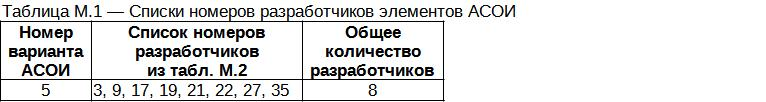
\includegraphics[]
            {_docs/ТаблицаМ1СпискиНомеровРазработчиковЭлементовАСОИ.jpg}
        \caption{Списки номеров разработчиков элементов АСОИ}
    \end{figure}

    \begin{figure}[ph!]
        \centering
        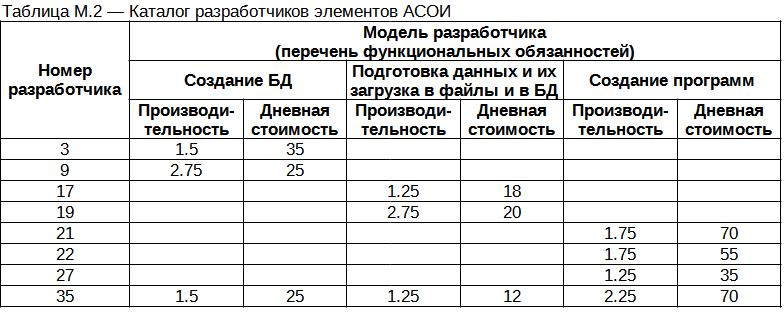
\includegraphics[width=16cm]
            {_docs/ТаблицаМ2КаталогРазработчиковЭлементовАСОИ.jpg}
        \caption{Таблица 3.1 - Характеристики разраотчиков программ}
    \end{figure}

    \begin{figure}[ph!]
        \centering
        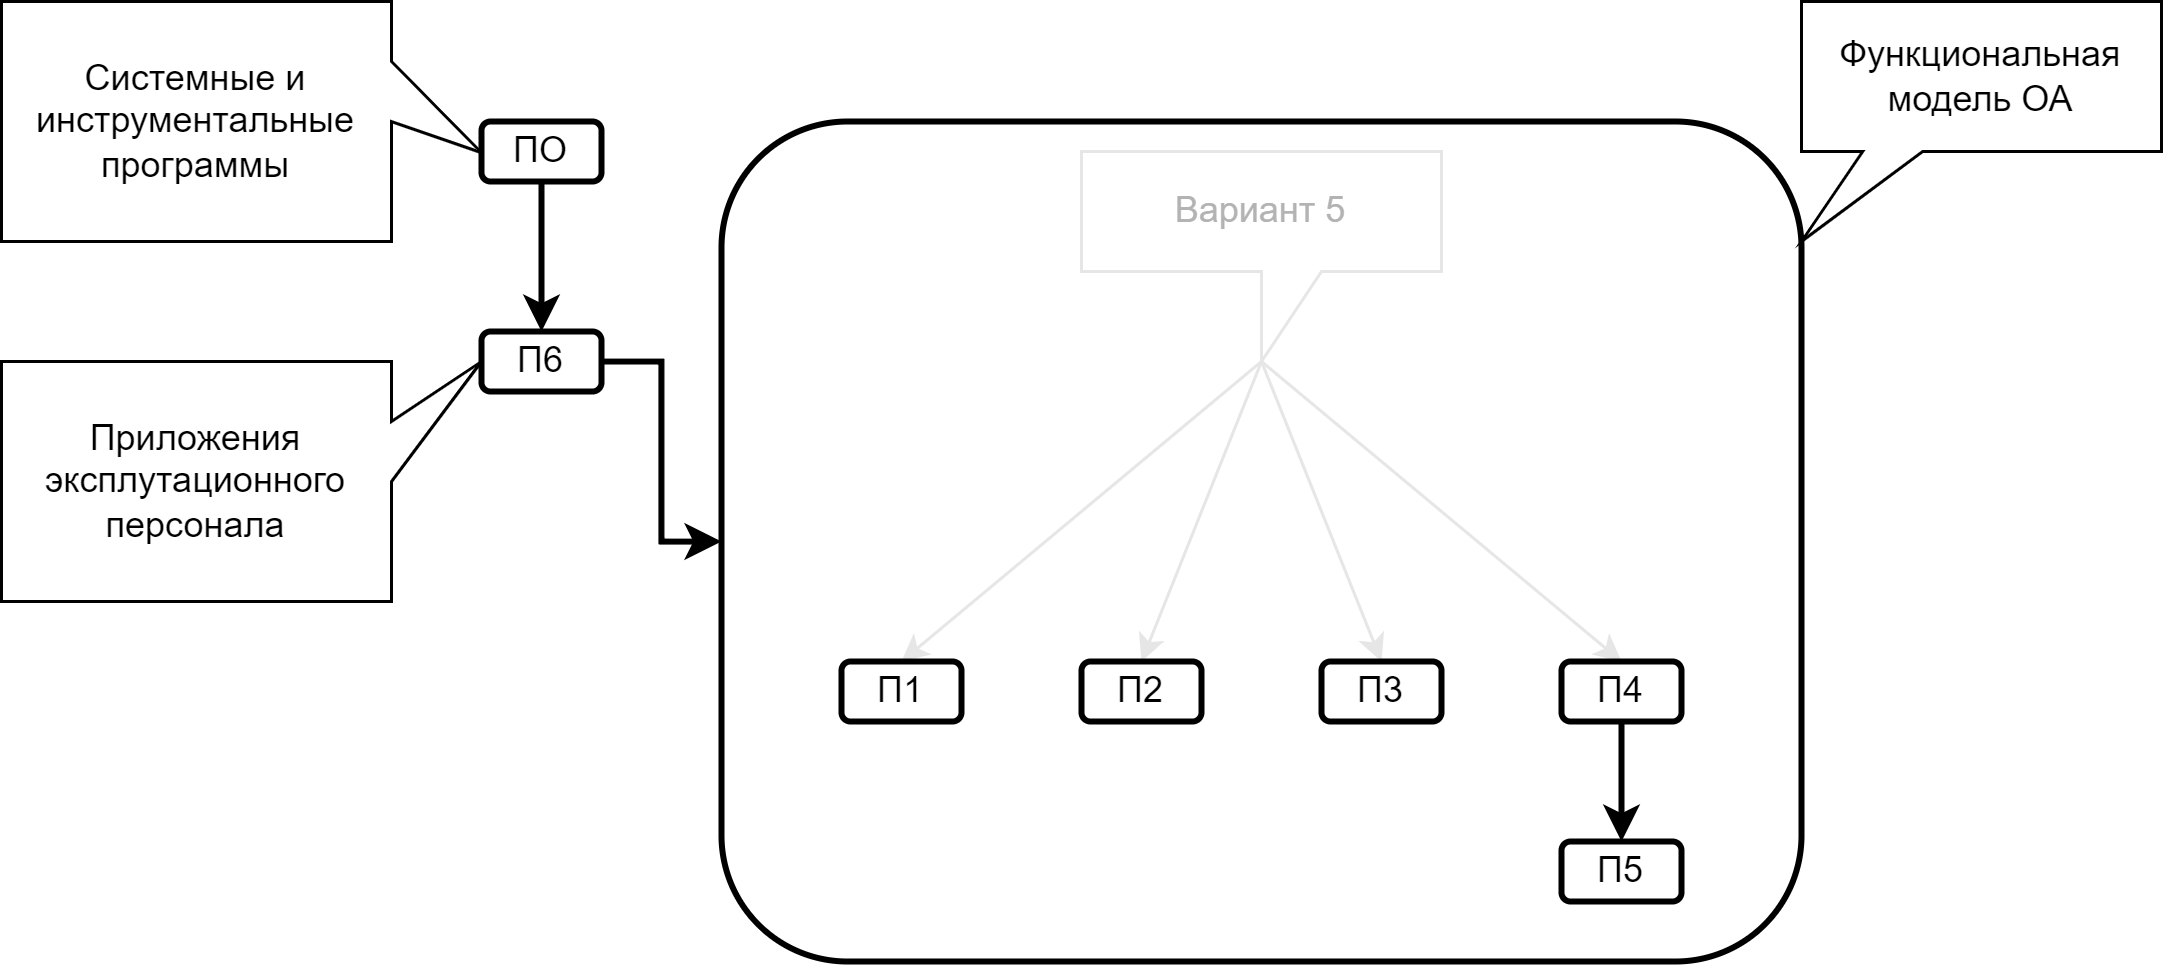
\includegraphics[width=16cm]
            {_docs/Рисунок3-1ПримерЛогическойСтруктурыПСАСОИ.png}
        \caption{Пример логической структуры ПС АСОИ}
    \end{figure}

\end{document}
